\documentclass[12pt,english,a4paper]{article}
\pdfobjcompresslevel=0
\usepackage[usenames,dvipsnames]{xcolor}
\usepackage[includeheadfoot,margin=0.8 in,top=0.6 in]{geometry}
\usepackage{siunitx,physics,cancel,upgreek,varioref,listings,booktabs,tocloft, pdfpages}
\usepackage{mathtools}
\usepackage{babel}
\usepackage{graphicx}
\usepackage{float}
\usepackage{fouriernc}
\usepackage{fancyhdr}
\usepackage[utf8]{inputenc}
\usepackage{amsmath}
\usepackage{amssymb}
\usepackage{textcomp}
\usepackage{lastpage}
\usepackage{microtype}
\usepackage[linktoc=all, bookmarks=true, pdfauthor={Anders Johansson}]{hyperref}
\renewcommand{\CancelColor}{\color{red}}
\renewcommand{\exp}[1]{\mathrm{e}^{#1}}
\newcommand{\R}{\mathbb{R}}
\newcommand{\tittel}[1]{\title{#1 \vspace{-7ex}}\author{}\date{}\maketitle\thispagestyle{fancy}\pagestyle{fancy}\setcounter{page}{1}}

\newcommand{\deloppg}[2][]{\subsection*{#2) #1}\addcontentsline{toc}{subsection}{#2)}\refstepcounter{subsection}\label{#2}}
\newcommand{\oppg}[1]{\section*{Oppgave #1}\addcontentsline{toc}{section}{Oppgave #1}\refstepcounter{section}\label{oppg#1}}

\labelformat{section}{section~#1}
\labelformat{subsection}{section~#1}
\labelformat{subsubsection}{paragraph~#1}
\labelformat{equation}{equation~(#1)}
\labelformat{figure}{figure~#1}
\labelformat{table}{table~#1}

\lstset{rangeprefix=/*\#,
rangesuffix=\#*/,
includerangemarker=false}
\renewcommand{\lstlistingname}{Code snippet}
\definecolor{codegreen}{rgb}{0,0.6,0}
\definecolor{codegray}{rgb}{0.5,0.5,0.5}
\definecolor{codepurple}{rgb}{0.58,0,0.82}
\definecolor{backcolour}{rgb}{0.95,0.95,0.92}
\lstset{showstringspaces=false,
basicstyle=\footnotesize\ttfamily,
keywordstyle=\color{codegreen},
commentstyle=\color{magenta},
numberstyle=\tiny\color{codegray},
stringstyle=\color{codepurple},
frameshape={RYRYNYYYY}{yny}{yny}{RYRYNYYYY},
breaklines=true,
%literate={0}{{\textcolor{blue}{0}}}{1}%
%             {1}{{\textcolor{blue}{1}}}{1}%
%             {2}{{\textcolor{blue}{2}}}{1}%
%             {3}{{\textcolor{blue}{3}}}{1}%
%             {4}{{\textcolor{blue}{4}}}{1}%
%             {5}{{\textcolor{blue}{5}}}{1}%
%             {6}{{\textcolor{blue}{6}}}{1}%
%             {7}{{\textcolor{blue}{7}}}{1}%
%             {8}{{\textcolor{blue}{8}}}{1}%
%             {9}{{\textcolor{blue}{9}}}{1}%
%             {.0}{{\textcolor{blue}{.0}}}{2}% Following is to ensure that only periods
%             {.1}{{\textcolor{blue}{.1}}}{2}% followed by a digit are changed.
%             {.2}{{\textcolor{blue}{.2}}}{2}%
%             {.3}{{\textcolor{blue}{.3}}}{2}%
%             {.4}{{\textcolor{blue}{.4}}}{2}%
%             {.5}{{\textcolor{blue}{.5}}}{2}%
%             {.6}{{\textcolor{blue}{.6}}}{2}%
%             {.7}{{\textcolor{blue}{.7}}}{2}%
%             {.8}{{\textcolor{blue}{.8}}}{2}%
%             {.9}{{\textcolor{blue}{.9}}}{2}%
}

\renewcommand{\footrulewidth}{\headrulewidth}
\tocloftpagestyle{fancy}

\setcounter{secnumdepth}{4}
\renewcommand{\thesection}{\arabic{section}}
\renewcommand{\thesubsection}{\arabic{section}.\arabic{subsection}}
\renewcommand{\thesubsubsection}{\arabic{section}.\arabic{subsection}.\arabic{subsubsection}}
\setlength{\parindent}{0cm}
\setlength{\parskip}{1em}

\newcommand{\eqtag}[1]{\refstepcounter{equation}\tag{\theequation}\label{#1}}
\hypersetup{colorlinks=true,urlcolor=blue,linkcolor=black}

\sisetup{detect-all}
\sisetup{exponent-product = \cdot, output-product = \cdot,per-mode=symbol}
\sisetup{output-decimal-marker={.}}
\sisetup{round-mode = off, round-precision=3}
\sisetup{number-unit-product = \ }
\DeclareSIUnit\year{yr}

\allowdisplaybreaks[4]
\fancyhf{}

\rhead{Anders Johansson}
\rfoot{Page \thepage{} of \pageref{LastPage}}
\lhead{FYS3150}
%
\usepackage[backend=biber,citestyle=numeric-comp,bibstyle=numeric,sorting=none]{biblatex}
\DefineBibliographyStrings{norsk}{%
  bibliography = {Referanser},
}
\DefineBibliographyStrings{english}{%
  bibliography = {References},
}
\addbibresource{kilder.bib}

\newcommand{\program}[1]{\href{https://github.com/anjohan/Offentlig/blob/master/FYS3150/Oblig3/#1}{#1}}

\begin{document}
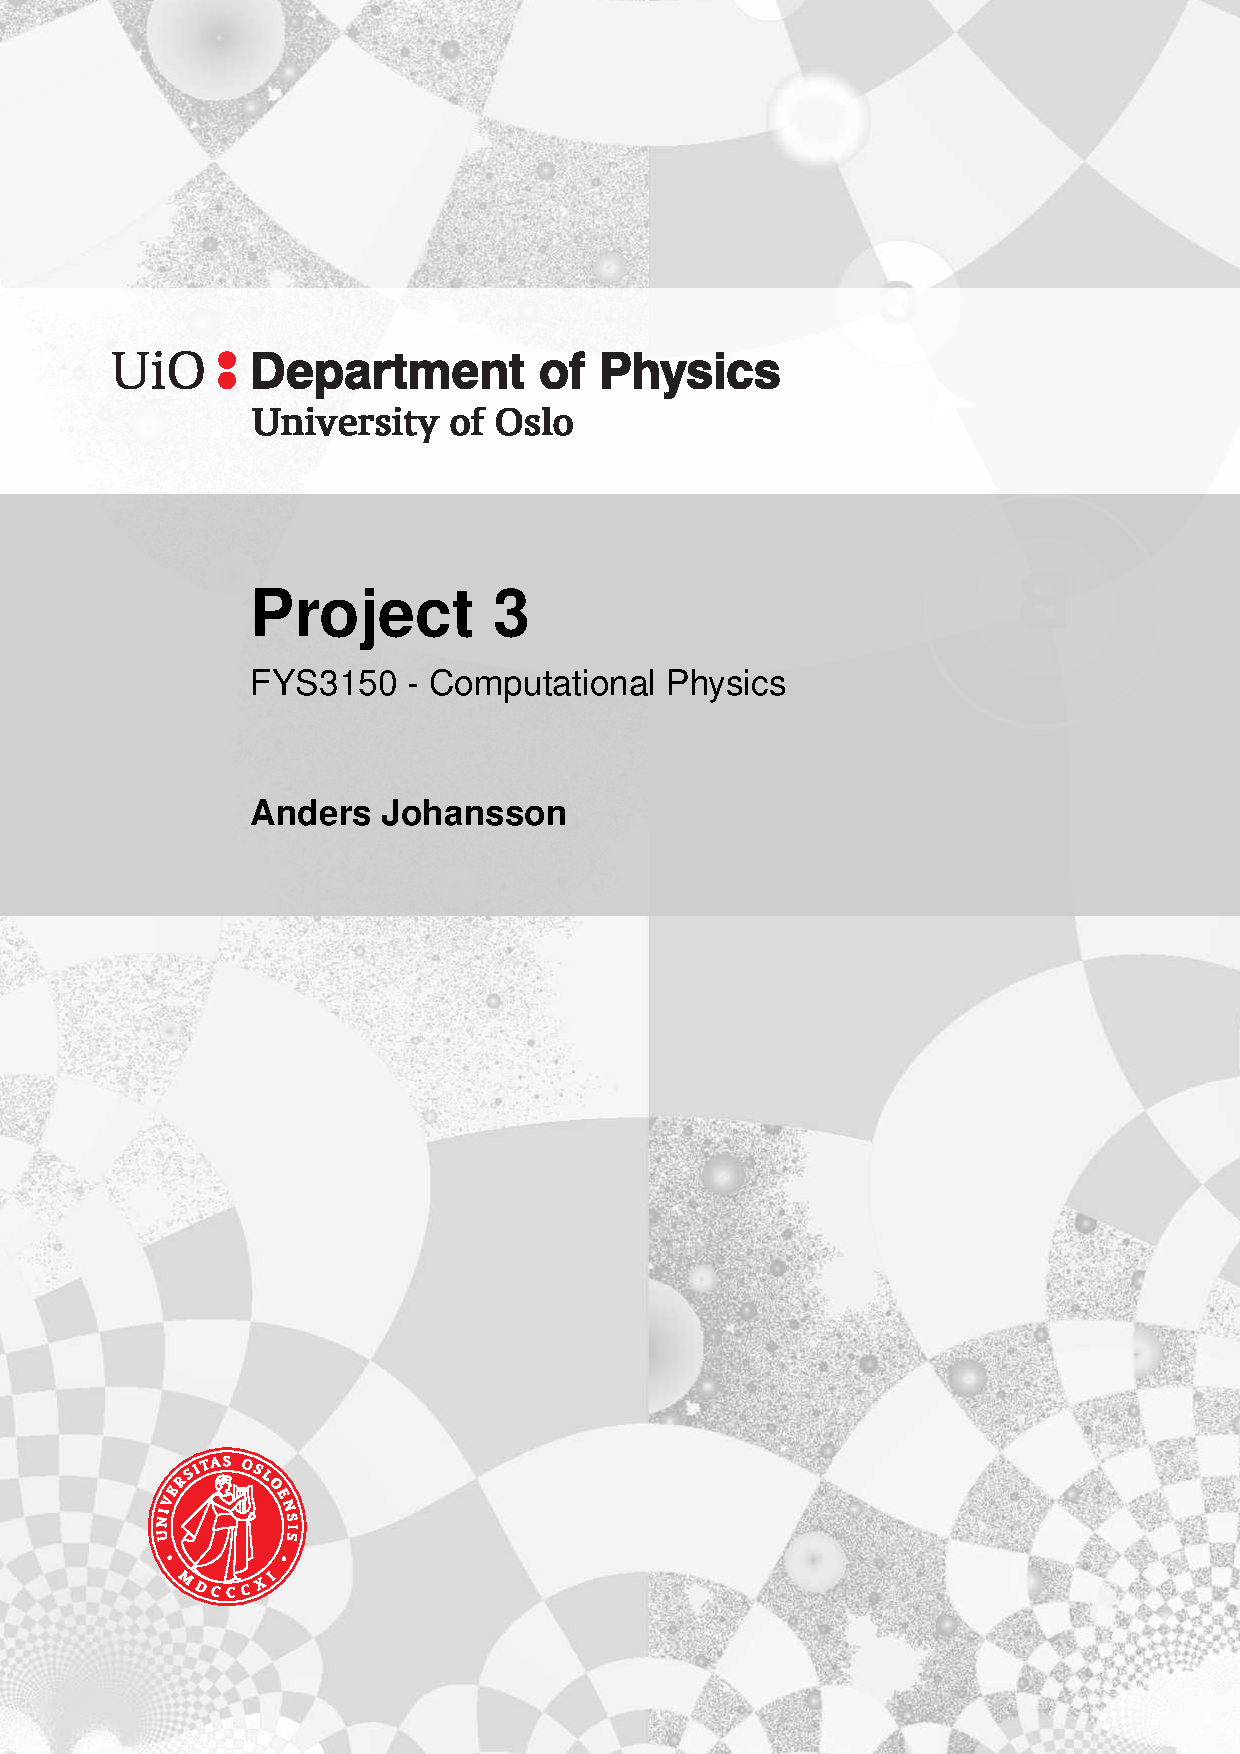
\includepdf{forside.pdf}
\pagestyle{fancy}
\tableofcontents

%      _             _
%  ___| |_ __ _ _ __| |_
% / __| __/ _` | '__| __|
% \__ \ || (_| | |  | |_
% |___/\__\__,_|_|   \__|
%

\begin{abstract}
In this project, various variations of solar systems are modelled using two different numerical algorithms for solving differential equations: The Forward Euler method and the Velocity-Verlet method. Both methods are derived with qualitative error analysis. The algorithms are applied to two, three and many body systems, with and without relativistic corrections and moving suns, in both two and three dimensions. Stability of the Verlet method is tested using a three body system with different mass ratios. The results coincide well with observed, elliptical orbits for the Verlet method, while the Forward Euler method proves to be insufficiently accurate. Benchmarking the algorithms shows that the theoretically predicted time ratio of \(\num{1.3}\) for a two body system fits quite well.
\end{abstract}



\clearpage
\section{Introduction}
Planets and their motion have fascinated mankind for millenia. Perhaps the biggest step forward came when Newton developed his gravitational law, which makes it possible to predict the motion of planets and other bodies only affected by gravitational forces. Then, in the beginning of the previous century, Einstein developed his theory of general relativity, which gave small corrections to Newton's model.

The existence of these laws is, however, not sufficient to know the position of the planets -- one also has to solve the equations, typically differential equations, that arise. This is often non-trivial, or even impossible, which means that numerical methods must once again be applied. The goal of this project is to solve the equations and predict the motion of the planets in our solar system.

In this project, both the most famous algorithm, the Forward Euler method, and one of the most used algorithms, the Velocity Verlet method, are derived and discussed. Their time usage and results are compared for the earth-sun-system, where the Verlet method proves its superior accuracy and ability to conserve momentum, energy and angular momentum, at the cost of a \(\SI{30}{\percent}\) increase in run time. The stability of the Verlet algorithm is then tested on three body systems with very different mass ratios, where the algorithm struggles to give realistic results. Then, the Verlet method is applied to all the planets in the solar system.

Finally, a relativistic correction is made to Newton's gravitational law. This causes the elliptic orbit of Mercury to rotate slightly, resulting in the so-called perihelion precession. The experimental results are verified.


%   __           _ _    _
%  / _|_   _ ___(_) | _| | __
% | |_| | | / __| | |/ / |/ /
% |  _| |_| \__ \ |   <|   <
% |_|  \__, |___/_|_|\_\_|\_\
%      |___/
\section{Physical theory}
\subsection{Gravitation}
In this project, a solar system will be studied. By solar system, I mean a system where only gravitational forces affect the bodies. Newtons gravitational law states that the gravitational force on a body with mass \(m\) from another body with mass \(M\) and relative position \(\vec{r}\) is given by\autocite{uniphys}:
\[
\vec{F}_\mathrm{G} = \frac{GmM}{\norm{\vec{r}}^2}\vec{r}
\]
where \(G\) is the gravitational constant, \(\SI{6.67e-11}{\N\meter\squared\per\second\squared}\). The direction of the force is given by the fact that gravity is an attractive force. If one of the objects is the sun, the mass is denoted by \(M_\odot\). With the sun placed in origo, \(r\) is simply the norm of the position vector of the planet with mass \(m\).

If there are \(n\) planets in the solar system, in addition to the sun, the sum of the forces on planet \(i\) with mass \(m_i\) is
\begin{alignat*}{2}
\sum{\vec{F}_i} &= \sum_{\substack{k=0\\k\neq i}}^n\frac{Gm_im_k}{\norm{\vec{r}_k-\vec{r}_i}^3}\qty(\vec{r}_k-\vec{r}_i)
\intertext{with \(m_0=M_\odot\) and \(\vec{r}_0=\vec{0}\). From Newton's second law, we know that \(\sum{\vec{F}_i}=m_i\vec{a}_i\), so the acceleration of planet \(i\) is given by}
\vec{a}_i &= \sum_{\substack{k=0\\k\neq i}}^n \frac{Gm_k}{\norm{\vec{r}_k-\vec{r}_i}^3}\qty(\vec{r}_k-\vec{r}_i) \eqtag{avec}
\end{alignat*}


%             _          _
%   ___ _ __ | |__   ___| |_ ___ _ __
%  / _ \ '_ \| '_ \ / _ \ __/ _ \ '__|
% |  __/ | | | | | |  __/ ||  __/ |
%  \___|_| |_|_| |_|\___|\__\___|_|
%
\subsection{Choice of units}
In the solar system, seconds and meters are unpractical, as planets are millions of kilometers apart and take years to do one lap around the sun. As such, it is common to use so-called astronomical units, where \(\SI{1}{\astronomicalunit}\) is the mean distance between the sun and the earth, and time is measured in years. To express the gravitational constant in these units, we can use that if the earth were moving in a circle around the sun, the acceleration in Newton's second law would be given by the sentripetal acceleration:
\[
\frac{mv^2}{r} = \frac{GmM_\odot}{r^2} \implies G = \frac{r}{M_\odot}v^2 = \frac{\SI{1}{\astronomicalunit}}{M_\odot} \cdot \qty(\frac{2\pi\cdot\SI{1}{\astronomicalunit}}{\SI{1}{\year}})^2 = \frac{4\pi^2}{M_\odot} \cdot  \SI{1}{\astronomicalunit\tothe3\per\year\squared}
\]
With this change of units, \vref{avec} can be written as
\[
\vec{a}_i = \sum_{\substack{k=0\\k\neq i}}^n 4\pi^2\frac{m_k}{M_\odot}\frac{\vec{r}_k-\vec{r}_i}{\norm{\vec{r}_k-\vec{r}_i}^3}\cdot \SI{1}{\astronomicalunit\cubed\per\year\squared} \eqtag{avecast}
\]

\subsection{Relativistic correction}
The preceding calculations use classical mechanics as developed by Newton. When taking the theory of general relativity into account, it can be shown\footnote{But not by me.} that the acceleration is given by
\[
\vec{a}_i = \sum_{\substack{k=0\\k\neq i}}^n 4\pi^2\frac{m_k}{M_\odot}\qty(1+\frac{3\norm{\vec{r}_i\times\vec{v}_i}^2}{\norm{\vec{r}_k-\vec{r}_i}^2c^2})\frac{\vec{r}_k-\vec{r}_i}{\norm{\vec{r}_k-\vec{r}_i}^3}\cdot \SI{1}{\astronomicalunit\cubed\per\year\squared} \eqtag{avecastrel}
\]
Note that the acceleration is no longer purely position dependent, so the Verlet method (see \vref{verlet}) can not be used exactly. However, approximating the Verlet method by using the old velocity should not be too bad an approximation.


%                  _                       _   _ _    _
%  _ __ ___   __ _| |_ ___ _ __ ___   __ _| |_(_) | _| | __
% | '_ ` _ \ / _` | __/ _ \ '_ ` _ \ / _` | __| | |/ / |/ /
% | | | | | | (_| | ||  __/ | | | | | (_| | |_| |   <|   <
% |_| |_| |_|\__,_|\__\___|_| |_| |_|\__,_|\__|_|_|\_\_|\_\
%

\section{Mathematical theory}
\Vref*{avecast}, together with some initial conditions, determines the motion of the bodies in the solar system. When written out in components, the equation gives a coupled set of differential equations. This set of equations is difficult, if at all possible, to solve analytically, so numerical work is required. As per usual, the time is discretised as \(t_i=t_0+ih\), where \(h\) is the time step, \(h=\qty(t_n-t_0)/n\). Acceleration, velocity and position are discretised correspondingly\autocite{oblig1}.


%             _
%   ___ _   _| | ___ _ __
%  / _ \ | | | |/ _ \ '__|
% |  __/ |_| | |  __/ |
%  \___|\__,_|_|\___|_|
%
\subsection{Forward Euler}
The Forward Euler method, also called the Explicit Euler method, and hereafter called simply the Euler method, uses a first order Taylor polynomial to approximate a solution to the diffrential equation. With \(x'(t)=v(t)\) and \(v'(t)=a(t)\), we have that
\begin{alignat*}{2}
\vec{r}_i(t+h)&\approx \vec{r}_i(t)+h\vec{v}_i(t)\\
\vec{v}_i(t+h)&\approx \vec{v}_i(t)+h\vec{a}_i(t)
\intertext{Discretised version:}
\vec{r}_{i,j+1} &\approx \vec{r}_{i,j} + h\vec{v}_{i,j}\\
\vec{v}_{i,j+1} &\approx \vec{v}_{i,j} + h\vec{a}_{i,j}
\end{alignat*}
To clarify the indices: \(\vec{a}_{i,j}\) is the acceleration of planet \(i\) at time step \(j\). This is calculated from \vref{avecast}.

From Taylor's formula, the error for a first order Taylor polynomial goes as \(O(h^2)\)\autocite{compphys}. This is the error made in each step --- the error is accumulated, so the total error will be proportional \(h\).


%                 _      _
% __   _____ _ __| | ___| |_
% \ \ / / _ \ '__| |/ _ \ __|
%  \ V /  __/ |  | |  __/ |_
%   \_/ \___|_|  |_|\___|\__|
%
\subsection{Velocity-Verlet}\label{verlet}
The Velocity-Verlet method, hereafter called the Verlet method, is based on a second order Taylor polynomial.
\begin{alignat*}{2}
\vec{r}_i(t+h) &\approx \vec{r}_i(t) + h\vec{v}_i(t) + \tfrac{1}{2}h^2\vec{a}_i(t)\\
\vec{v}_i(t+h) &\approx \vec{v}_i(t) + h\vec{a}_i(t) + \tfrac{1}{2}h^2\vec{a}_i'(t)
\end{alignat*}
There is no explicit expression for \(\vec{a}'(t)\), however it can be approximated using the good old formula
\[
\vec{a}'(t)\approx\frac{\vec{a}(t+h)-\vec{a}(t)}{h}
\]
Since the acceleration is independent of the velocity, the newly updated position, \(\vec{a}(t+h)\), can be calculated using \(\vec{r}(t+h)\). Inserting this into the expression for \(\vec{v}(t+h)\), we get
\begin{alignat*}{2}
\vec{v}_i(t+h) &\approx \vec{v}_i(t) + h\vec{a}_i(t) + \tfrac{1}{2}h\qty(\vec{a}_i(t+h)-\vec{a}_i(t))\\
&= \vec{v}_i(t) + \tfrac{1}{2}h\qty(\vec{a}_i(t)+\vec{a}_i(t+h))
\end{alignat*}
The discretised version then becomes
\begin{alignat*}{2}
\vec{r}_{i,j+1} &\approx \vec{r}_{i,j} + h\vec{v}_{i,j} + \tfrac{1}{2}h^2\vec{a}_{i,j}\\
\vec{v}_{i,j+1} &\approx \vec{v}_{i,j} + \tfrac{1}{2}h\qty(\vec{a}_{i,j} + \vec{a}_{i,j+1})
\end{alignat*}
The error of a second order Taylor polynomial is given as \(O(h^3)\). The approximation for \(\vec{a}'(t)\) has an error proportional to \(h\), but this error is multiplied with \(h^2\) when inserted into the expression for \(\vec{v}_i(t+h)\). As such, the error for each step is proportional to \(h^3\)\autocite{compphys}. The error is again accumulated for each step, so the total error will be proportional to \(h^2\). This is one order better than the Euler method.


%  _                 _                           _             _
% (_)_ __ ___  _ __ | | ___ _ __ ___   ___ _ __ | |_ __ _ ___ (_) ___  _ __
% | | '_ ` _ \| '_ \| |/ _ \ '_ ` _ \ / _ \ '_ \| __/ _` / __|| |/ _ \| '_ \
% | | | | | | | |_) | |  __/ | | | | |  __/ | | | || (_| \__ \| | (_) | | | |
% |_|_| |_| |_| .__/|_|\___|_| |_| |_|\___|_| |_|\__\__,_|___// |\___/|_| |_|
%             |_|                                           |__/
\section{Implementation}
The implementation is heavily object oriented and modular by design. The \texttt{Planet} class (\program{planet.h} and \program{planet.cpp}) represents a body, with methods for calculating the acceleration according to \ref{avecast} as well as updating position and velocity for both algorithms. The \texttt{SolarSystem} class (\program{solarsystem.h} and \program{solarsystem.cpp}) administrates the planets, and contains a method for each algorithm. \program{cpp\_ui.cpp} sets up the solar system according to the command line arguments, and calls the solver method specified. \program{python\_ui.py} is a user-friendly interface to \program{cpp\_ui.cpp}, see \program{README.md}.

\program{conservation.py} is a Python program that reads a data file and checks that momentum, energy and angular momentum are conserved. As there are no external forces (or torques) acting on the solar system, these quantities should always be conserved. Note that this program is not intended to be read.

The relativistic correction can not be run with \program{python\_ui.py} - this must be run manually. See \program{perihelion.cpp} for an example. \texttt{PerihelionFinder} and its subclass \texttt{RelativisticPlanet} have overloaded methods for this purpose.

In my implementation, the data is stored by writing to file. This means that the simulation requires less than 150 kB of memory, which is very positive. The amount of data written to file can easily be controlled through the \texttt{dn} parameter.

\subsection{Number of floating point operations (FLOPs)}
\renewcommand{\theenumii}{\arabic{enumii}}
\renewcommand{\theenumiii}{\arabic{enumiii}}
To calculate the acceleration (common for both algorithms):
\begin{itemize}
\item For each of the \(n\) planets:
\begin{itemize}
\item For each of the \(n-1\) other planets:
\begin{enumerate}
\item Subtract the \(x\), \(y\) and \(z\) components (3 FLOPs).
\item Square the differences in the \(x\), \(y\) and \(z\) components (3 FLOPs).
\item Add these differences (2 FLOPs).
\item Take the square root (1 FLOP\footnote{Or possibly more.}).
\item Calculate the cube of the norm (2 FLOPs).
\item Divide \(4\pi^2\) times the mass ratio (precalculated) by the cube of the norm (1 FLOP).\label{factor}
\item Multiply this factor by the differences in \(x\), \(y\) and \(z\) positions (3 FLOPs).
\item Add these to the \(x\), \(y\) and \(z\) components of the acceleration (3 FLOP).
\end{enumerate}
\end{itemize}
\end{itemize}
\(18n\qty(n-1)\) floating point operations in total.

\textbf{For the Euler method:}
\begin{itemize}
\item For each of the \(n\) planets:
\begin{enumerate}
\item Multiply the \(x\), \(y\) and \(z\) components of the acceleration with the time step (3 FLOPs).
\item Add these to the \(x\), \(y\) and \(z\) components of the velocity (3 FLOPs).
\item Multiply the \(x\), \(y\) and \(z\) components of the velocity with the timestep (3 FLOPs).
\item Add these to the \(x\), \(y\) and \(z\) components of the position (3 FLOPs).
\end{enumerate}
\item Calculate the acceleration (\(18n\qty(n-1)\) FLOPs).
\end{itemize}
This gives a total of \[12n + 18n\qty(n-1) = 18n^2-6n\eqtag{eulerflops}\] floating point operations per time step.

\textbf{For the Verlet method:}
\begin{itemize}
\item For each of the \(n\) planets:
\begin{enumerate}
\item Multiply the time step with the \(x\), \(y\) and \(z\) components of the velocity (3 FLOPs).
\item Multiply half the square of the time step (precalculated) with the \(x\), \(y\) and \(z\) components of the acceleration (3 FLOPs).
\item Add these to the \(x\), \(y\) and \(z\) components of the position (6 FLOPs).
\end{enumerate}
\item Calculate the new acceleration (\(18n\qty(n-1)\) FLOPs).
\item For each of the \(n\) planets:
\begin{enumerate}
\item Add the \(x\), \(y\) and \(z\) components of the new and old accelerations (3 FLOPs).
\item Multiply these by half the time step (precalculated) (3 FLOPs).
\item Add the results to the \(x\), \(y\) and \(z\) components of the velocity (3 FLOPs).
\item Set the new acceleration to be the old acceleration, and set the new acceleration to \(\vec{0}\) (0 FLOPs).
\end{enumerate}
\end{itemize}
This gives a total of \[12n + 18n\qty(n-1) + 9n = 18n^2+3n\eqtag{verletflops}\] floating point operations per time step.

%                      _ _        _
%  _ __ ___  ___ _   _| | |_ __ _| |_ ___ _ __
% | '__/ _ \/ __| | | | | __/ _` | __/ _ \ '__|
% | | |  __/\__ \ |_| | | || (_| | ||  __/ |
% |_|  \___||___/\__,_|_|\__\__,_|\__\___|_|
%
\section{Simulations and results}
\subsection{Earth-sun-system}
\begin{figure}[H]
\centering
% GNUPLOT: LaTeX picture with Postscript
\begingroup
  \makeatletter
  \providecommand\color[2][]{%
    \GenericError{(gnuplot) \space\space\space\@spaces}{%
      Package color not loaded in conjunction with
      terminal option `colourtext'%
    }{See the gnuplot documentation for explanation.%
    }{Either use 'blacktext' in gnuplot or load the package
      color.sty in LaTeX.}%
    \renewcommand\color[2][]{}%
  }%
  \providecommand\includegraphics[2][]{%
    \GenericError{(gnuplot) \space\space\space\@spaces}{%
      Package graphicx or graphics not loaded%
    }{See the gnuplot documentation for explanation.%
    }{The gnuplot epslatex terminal needs graphicx.sty or graphics.sty.}%
    \renewcommand\includegraphics[2][]{}%
  }%
  \providecommand\rotatebox[2]{#2}%
  \@ifundefined{ifGPcolor}{%
    \newif\ifGPcolor
    \GPcolortrue
  }{}%
  \@ifundefined{ifGPblacktext}{%
    \newif\ifGPblacktext
    \GPblacktextfalse
  }{}%
  % define a \g@addto@macro without @ in the name:
  \let\gplgaddtomacro\g@addto@macro
  % define empty templates for all commands taking text:
  \gdef\gplbacktext{}%
  \gdef\gplfronttext{}%
  \makeatother
  \ifGPblacktext
    % no textcolor at all
    \def\colorrgb#1{}%
    \def\colorgray#1{}%
  \else
    % gray or color?
    \ifGPcolor
      \def\colorrgb#1{\color[rgb]{#1}}%
      \def\colorgray#1{\color[gray]{#1}}%
      \expandafter\def\csname LTw\endcsname{\color{white}}%
      \expandafter\def\csname LTb\endcsname{\color{black}}%
      \expandafter\def\csname LTa\endcsname{\color{black}}%
      \expandafter\def\csname LT0\endcsname{\color[rgb]{1,0,0}}%
      \expandafter\def\csname LT1\endcsname{\color[rgb]{0,1,0}}%
      \expandafter\def\csname LT2\endcsname{\color[rgb]{0,0,1}}%
      \expandafter\def\csname LT3\endcsname{\color[rgb]{1,0,1}}%
      \expandafter\def\csname LT4\endcsname{\color[rgb]{0,1,1}}%
      \expandafter\def\csname LT5\endcsname{\color[rgb]{1,1,0}}%
      \expandafter\def\csname LT6\endcsname{\color[rgb]{0,0,0}}%
      \expandafter\def\csname LT7\endcsname{\color[rgb]{1,0.3,0}}%
      \expandafter\def\csname LT8\endcsname{\color[rgb]{0.5,0.5,0.5}}%
    \else
      % gray
      \def\colorrgb#1{\color{black}}%
      \def\colorgray#1{\color[gray]{#1}}%
      \expandafter\def\csname LTw\endcsname{\color{white}}%
      \expandafter\def\csname LTb\endcsname{\color{black}}%
      \expandafter\def\csname LTa\endcsname{\color{black}}%
      \expandafter\def\csname LT0\endcsname{\color{black}}%
      \expandafter\def\csname LT1\endcsname{\color{black}}%
      \expandafter\def\csname LT2\endcsname{\color{black}}%
      \expandafter\def\csname LT3\endcsname{\color{black}}%
      \expandafter\def\csname LT4\endcsname{\color{black}}%
      \expandafter\def\csname LT5\endcsname{\color{black}}%
      \expandafter\def\csname LT6\endcsname{\color{black}}%
      \expandafter\def\csname LT7\endcsname{\color{black}}%
      \expandafter\def\csname LT8\endcsname{\color{black}}%
    \fi
  \fi
    \setlength{\unitlength}{0.0500bp}%
    \ifx\gptboxheight\undefined%
      \newlength{\gptboxheight}%
      \newlength{\gptboxwidth}%
      \newsavebox{\gptboxtext}%
    \fi%
    \setlength{\fboxrule}{0.5pt}%
    \setlength{\fboxsep}{1pt}%
\begin{picture}(5760.00,5760.00)%
    \gplgaddtomacro\gplbacktext{%
      \csname LTb\endcsname%
      \put(946,704){\makebox(0,0)[r]{\strut{}$-1.5$}}%
      \put(946,1503){\makebox(0,0)[r]{\strut{}$-1$}}%
      \put(946,2301){\makebox(0,0)[r]{\strut{}$-0.5$}}%
      \put(946,3100){\makebox(0,0)[r]{\strut{}$0$}}%
      \put(946,3898){\makebox(0,0)[r]{\strut{}$0.5$}}%
      \put(946,4697){\makebox(0,0)[r]{\strut{}$1$}}%
      \put(946,5495){\makebox(0,0)[r]{\strut{}$1.5$}}%
      \put(1078,484){\makebox(0,0){\strut{}$-1.5$}}%
      \put(1792,484){\makebox(0,0){\strut{}$-1$}}%
      \put(2506,484){\makebox(0,0){\strut{}$-0.5$}}%
      \put(3221,484){\makebox(0,0){\strut{}$0$}}%
      \put(3935,484){\makebox(0,0){\strut{}$0.5$}}%
      \put(4649,484){\makebox(0,0){\strut{}$1$}}%
      \put(5363,484){\makebox(0,0){\strut{}$1.5$}}%
    }%
    \gplgaddtomacro\gplfronttext{%
      \csname LTb\endcsname%
      \put(176,3099){\rotatebox{-270}{\makebox(0,0){\strut{}$y\ [\si{\astronomicalunit}]$}}}%
      \put(3220,154){\makebox(0,0){\strut{}$x\ [\si{\astronomicalunit}]$}}%
      \csname LTb\endcsname%
      \put(4376,5322){\makebox(0,0)[r]{\strut{}Sun, Euler}}%
      \csname LTb\endcsname%
      \put(4376,5102){\makebox(0,0)[r]{\strut{}Earth, Euler}}%
      \csname LTb\endcsname%
      \put(4376,4882){\makebox(0,0)[r]{\strut{}Sun, Verlet}}%
      \csname LTb\endcsname%
      \put(4376,4662){\makebox(0,0)[r]{\strut{}Earth, Verlet}}%
    }%
    \gplbacktext
    \put(0,0){\includegraphics{earthsun}}%
    \gplfronttext
  \end{picture}%
\endgroup

\caption{Simulation of the earth-sun-system with both the Forward Euler and the Velocity-Verlet algorithms. The simulation was run for \(1\) year with \(\num{1000}\) integration points, which clearly is insufficient for the Forward Euler method. The simulation was run by \program{earthsun.sh}.}
\end{figure}

\subsubsection{Visual error analysis}
When given a tangential velocity of \(2\pi\ \si{\astronomicalunit\per\year}\), the earth should return to its initial position after one year.
\begin{figure}[H]
\centering
% GNUPLOT: LaTeX picture with Postscript
\begingroup
  \makeatletter
  \providecommand\color[2][]{%
    \GenericError{(gnuplot) \space\space\space\@spaces}{%
      Package color not loaded in conjunction with
      terminal option `colourtext'%
    }{See the gnuplot documentation for explanation.%
    }{Either use 'blacktext' in gnuplot or load the package
      color.sty in LaTeX.}%
    \renewcommand\color[2][]{}%
  }%
  \providecommand\includegraphics[2][]{%
    \GenericError{(gnuplot) \space\space\space\@spaces}{%
      Package graphicx or graphics not loaded%
    }{See the gnuplot documentation for explanation.%
    }{The gnuplot epslatex terminal needs graphicx.sty or graphics.sty.}%
    \renewcommand\includegraphics[2][]{}%
  }%
  \providecommand\rotatebox[2]{#2}%
  \@ifundefined{ifGPcolor}{%
    \newif\ifGPcolor
    \GPcolortrue
  }{}%
  \@ifundefined{ifGPblacktext}{%
    \newif\ifGPblacktext
    \GPblacktextfalse
  }{}%
  % define a \g@addto@macro without @ in the name:
  \let\gplgaddtomacro\g@addto@macro
  % define empty templates for all commands taking text:
  \gdef\gplbacktext{}%
  \gdef\gplfronttext{}%
  \makeatother
  \ifGPblacktext
    % no textcolor at all
    \def\colorrgb#1{}%
    \def\colorgray#1{}%
  \else
    % gray or color?
    \ifGPcolor
      \def\colorrgb#1{\color[rgb]{#1}}%
      \def\colorgray#1{\color[gray]{#1}}%
      \expandafter\def\csname LTw\endcsname{\color{white}}%
      \expandafter\def\csname LTb\endcsname{\color{black}}%
      \expandafter\def\csname LTa\endcsname{\color{black}}%
      \expandafter\def\csname LT0\endcsname{\color[rgb]{1,0,0}}%
      \expandafter\def\csname LT1\endcsname{\color[rgb]{0,1,0}}%
      \expandafter\def\csname LT2\endcsname{\color[rgb]{0,0,1}}%
      \expandafter\def\csname LT3\endcsname{\color[rgb]{1,0,1}}%
      \expandafter\def\csname LT4\endcsname{\color[rgb]{0,1,1}}%
      \expandafter\def\csname LT5\endcsname{\color[rgb]{1,1,0}}%
      \expandafter\def\csname LT6\endcsname{\color[rgb]{0,0,0}}%
      \expandafter\def\csname LT7\endcsname{\color[rgb]{1,0.3,0}}%
      \expandafter\def\csname LT8\endcsname{\color[rgb]{0.5,0.5,0.5}}%
    \else
      % gray
      \def\colorrgb#1{\color{black}}%
      \def\colorgray#1{\color[gray]{#1}}%
      \expandafter\def\csname LTw\endcsname{\color{white}}%
      \expandafter\def\csname LTb\endcsname{\color{black}}%
      \expandafter\def\csname LTa\endcsname{\color{black}}%
      \expandafter\def\csname LT0\endcsname{\color{black}}%
      \expandafter\def\csname LT1\endcsname{\color{black}}%
      \expandafter\def\csname LT2\endcsname{\color{black}}%
      \expandafter\def\csname LT3\endcsname{\color{black}}%
      \expandafter\def\csname LT4\endcsname{\color{black}}%
      \expandafter\def\csname LT5\endcsname{\color{black}}%
      \expandafter\def\csname LT6\endcsname{\color{black}}%
      \expandafter\def\csname LT7\endcsname{\color{black}}%
      \expandafter\def\csname LT8\endcsname{\color{black}}%
    \fi
  \fi
    \setlength{\unitlength}{0.0500bp}%
    \ifx\gptboxheight\undefined%
      \newlength{\gptboxheight}%
      \newlength{\gptboxwidth}%
      \newsavebox{\gptboxtext}%
    \fi%
    \setlength{\fboxrule}{0.5pt}%
    \setlength{\fboxsep}{1pt}%
\begin{picture}(7200.00,5760.00)%
    \gplgaddtomacro\gplbacktext{%
      \csname LTb\endcsname%
      \put(946,704){\makebox(0,0)[r]{\strut{}$-1.8$}}%
      \csname LTb\endcsname%
      \put(946,1183){\makebox(0,0)[r]{\strut{}$-1.6$}}%
      \csname LTb\endcsname%
      \put(946,1662){\makebox(0,0)[r]{\strut{}$-1.4$}}%
      \csname LTb\endcsname%
      \put(946,2141){\makebox(0,0)[r]{\strut{}$-1.2$}}%
      \csname LTb\endcsname%
      \put(946,2620){\makebox(0,0)[r]{\strut{}$-1$}}%
      \csname LTb\endcsname%
      \put(946,3099){\makebox(0,0)[r]{\strut{}$-0.8$}}%
      \csname LTb\endcsname%
      \put(946,3579){\makebox(0,0)[r]{\strut{}$-0.6$}}%
      \csname LTb\endcsname%
      \put(946,4058){\makebox(0,0)[r]{\strut{}$-0.4$}}%
      \csname LTb\endcsname%
      \put(946,4537){\makebox(0,0)[r]{\strut{}$-0.2$}}%
      \csname LTb\endcsname%
      \put(946,5016){\makebox(0,0)[r]{\strut{}$0$}}%
      \csname LTb\endcsname%
      \put(946,5495){\makebox(0,0)[r]{\strut{}$0.2$}}%
      \csname LTb\endcsname%
      \put(1078,484){\makebox(0,0){\strut{}$-0.6$}}%
      \csname LTb\endcsname%
      \put(1714,484){\makebox(0,0){\strut{}$-0.4$}}%
      \csname LTb\endcsname%
      \put(2350,484){\makebox(0,0){\strut{}$-0.2$}}%
      \csname LTb\endcsname%
      \put(2986,484){\makebox(0,0){\strut{}$0$}}%
      \csname LTb\endcsname%
      \put(3622,484){\makebox(0,0){\strut{}$0.2$}}%
      \csname LTb\endcsname%
      \put(4259,484){\makebox(0,0){\strut{}$0.4$}}%
      \csname LTb\endcsname%
      \put(4895,484){\makebox(0,0){\strut{}$0.6$}}%
      \csname LTb\endcsname%
      \put(5531,484){\makebox(0,0){\strut{}$0.8$}}%
      \csname LTb\endcsname%
      \put(6167,484){\makebox(0,0){\strut{}$1$}}%
      \csname LTb\endcsname%
      \put(6803,484){\makebox(0,0){\strut{}$1.2$}}%
    }%
    \gplgaddtomacro\gplfronttext{%
      \csname LTb\endcsname%
      \put(176,3099){\rotatebox{-270}{\makebox(0,0){\strut{}$y\ [\si{\astronomicalunit}]$}}}%
      \put(3940,154){\makebox(0,0){\strut{}$x\ [\si{\astronomicalunit}]$}}%
      \csname LTb\endcsname%
      \put(2002,5322){\makebox(0,0)[r]{\strut{}Euler}}%
      \csname LTb\endcsname%
      \put(2002,5102){\makebox(0,0)[r]{\strut{}Verlet}}%
    }%
    \gplbacktext
    \put(0,0){\includegraphics{error}}%
    \gplfronttext
  \end{picture}%
\endgroup

\caption{The end point of the earth after simulating for one year, with \(10^n\) timesteps for \(n=2,3,\dots\). It is clear that the Verlet method converges much more quickly than Euler's method. The data is generated by \program{errorearthsun.sh}.}
\end{figure}

\subsubsection{Benchmarks}
\begin{table}[H]
\caption{Benchmarks for both algorithms for the earth-sun-system. Generated by \program{timetable.py}.}
\centering
\input{timetable.dat}
\end{table}
The time grows very linearly as a function of the number of time steps, as expected.

With \(n=2\) (the number of planets), \ref{eulerflops} and \ref{verletflops} predict that the ratio between the times should be
\[
\frac{18\cdot2^2+3\cdot2}{18\cdot2^2-6\cdot2} = \frac{78}{60}=\num{1.3}
\]
This fits reasonably well with the tabulated data. The slightly lower observed ratio is probably caused by the fact that floating point operations do not take up all of the time --- some time is also spent on function calls, if-tests etc. Additionally, the square root might require more than one floating point operation.

\subsubsection{Conservation tests}
Running the command \texttt{python conservation.py earthsunverlet.dat} yields
\lstinputlisting[language={},frame=none]{earthsunverlettest.dat}
while \texttt{python conservation.py earthsuneuler.dat} yields
\lstinputlisting[language={},frame=none]{earthsuneulertest.dat}

\subsubsection{Escape speed}
The basis for sending stuff to other solar systems, is the possibility of escaping the sun's gravitational field. To to this, the total energy (potential and kinetic) must be greater than \(0\), as this means the object will have a positive kinetic energy even after moving infinitely far away from the sun (where the potential energy is 0).



\subsection{Three-body-problem with fixed sun and varying masses}
\begin{figure}[H]
\centering
% GNUPLOT: LaTeX picture with Postscript
\begingroup
  \makeatletter
  \providecommand\color[2][]{%
    \GenericError{(gnuplot) \space\space\space\@spaces}{%
      Package color not loaded in conjunction with
      terminal option `colourtext'%
    }{See the gnuplot documentation for explanation.%
    }{Either use 'blacktext' in gnuplot or load the package
      color.sty in LaTeX.}%
    \renewcommand\color[2][]{}%
  }%
  \providecommand\includegraphics[2][]{%
    \GenericError{(gnuplot) \space\space\space\@spaces}{%
      Package graphicx or graphics not loaded%
    }{See the gnuplot documentation for explanation.%
    }{The gnuplot epslatex terminal needs graphicx.sty or graphics.sty.}%
    \renewcommand\includegraphics[2][]{}%
  }%
  \providecommand\rotatebox[2]{#2}%
  \@ifundefined{ifGPcolor}{%
    \newif\ifGPcolor
    \GPcolortrue
  }{}%
  \@ifundefined{ifGPblacktext}{%
    \newif\ifGPblacktext
    \GPblacktextfalse
  }{}%
  % define a \g@addto@macro without @ in the name:
  \let\gplgaddtomacro\g@addto@macro
  % define empty templates for all commands taking text:
  \gdef\gplbacktext{}%
  \gdef\gplfronttext{}%
  \makeatother
  \ifGPblacktext
    % no textcolor at all
    \def\colorrgb#1{}%
    \def\colorgray#1{}%
  \else
    % gray or color?
    \ifGPcolor
      \def\colorrgb#1{\color[rgb]{#1}}%
      \def\colorgray#1{\color[gray]{#1}}%
      \expandafter\def\csname LTw\endcsname{\color{white}}%
      \expandafter\def\csname LTb\endcsname{\color{black}}%
      \expandafter\def\csname LTa\endcsname{\color{black}}%
      \expandafter\def\csname LT0\endcsname{\color[rgb]{1,0,0}}%
      \expandafter\def\csname LT1\endcsname{\color[rgb]{0,1,0}}%
      \expandafter\def\csname LT2\endcsname{\color[rgb]{0,0,1}}%
      \expandafter\def\csname LT3\endcsname{\color[rgb]{1,0,1}}%
      \expandafter\def\csname LT4\endcsname{\color[rgb]{0,1,1}}%
      \expandafter\def\csname LT5\endcsname{\color[rgb]{1,1,0}}%
      \expandafter\def\csname LT6\endcsname{\color[rgb]{0,0,0}}%
      \expandafter\def\csname LT7\endcsname{\color[rgb]{1,0.3,0}}%
      \expandafter\def\csname LT8\endcsname{\color[rgb]{0.5,0.5,0.5}}%
    \else
      % gray
      \def\colorrgb#1{\color{black}}%
      \def\colorgray#1{\color[gray]{#1}}%
      \expandafter\def\csname LTw\endcsname{\color{white}}%
      \expandafter\def\csname LTb\endcsname{\color{black}}%
      \expandafter\def\csname LTa\endcsname{\color{black}}%
      \expandafter\def\csname LT0\endcsname{\color{black}}%
      \expandafter\def\csname LT1\endcsname{\color{black}}%
      \expandafter\def\csname LT2\endcsname{\color{black}}%
      \expandafter\def\csname LT3\endcsname{\color{black}}%
      \expandafter\def\csname LT4\endcsname{\color{black}}%
      \expandafter\def\csname LT5\endcsname{\color{black}}%
      \expandafter\def\csname LT6\endcsname{\color{black}}%
      \expandafter\def\csname LT7\endcsname{\color{black}}%
      \expandafter\def\csname LT8\endcsname{\color{black}}%
    \fi
  \fi
    \setlength{\unitlength}{0.0500bp}%
    \ifx\gptboxheight\undefined%
      \newlength{\gptboxheight}%
      \newlength{\gptboxwidth}%
      \newsavebox{\gptboxtext}%
    \fi%
    \setlength{\fboxrule}{0.5pt}%
    \setlength{\fboxsep}{1pt}%
\begin{picture}(7200.00,7200.00)%
    \gplgaddtomacro\gplbacktext{%
      \csname LTb\endcsname%
      \put(682,704){\makebox(0,0)[r]{\strut{}$-6$}}%
      \csname LTb\endcsname%
      \put(682,1483){\makebox(0,0)[r]{\strut{}$-4$}}%
      \csname LTb\endcsname%
      \put(682,2262){\makebox(0,0)[r]{\strut{}$-2$}}%
      \csname LTb\endcsname%
      \put(682,3041){\makebox(0,0)[r]{\strut{}$0$}}%
      \csname LTb\endcsname%
      \put(682,3820){\makebox(0,0)[r]{\strut{}$2$}}%
      \csname LTb\endcsname%
      \put(682,4598){\makebox(0,0)[r]{\strut{}$4$}}%
      \csname LTb\endcsname%
      \put(682,5377){\makebox(0,0)[r]{\strut{}$6$}}%
      \csname LTb\endcsname%
      \put(682,6156){\makebox(0,0)[r]{\strut{}$8$}}%
      \csname LTb\endcsname%
      \put(682,6935){\makebox(0,0)[r]{\strut{}$10$}}%
      \csname LTb\endcsname%
      \put(814,484){\makebox(0,0){\strut{}$-6$}}%
      \csname LTb\endcsname%
      \put(1563,484){\makebox(0,0){\strut{}$-4$}}%
      \csname LTb\endcsname%
      \put(2311,484){\makebox(0,0){\strut{}$-2$}}%
      \csname LTb\endcsname%
      \put(3060,484){\makebox(0,0){\strut{}$0$}}%
      \csname LTb\endcsname%
      \put(3809,484){\makebox(0,0){\strut{}$2$}}%
      \csname LTb\endcsname%
      \put(4557,484){\makebox(0,0){\strut{}$4$}}%
      \csname LTb\endcsname%
      \put(5306,484){\makebox(0,0){\strut{}$6$}}%
      \csname LTb\endcsname%
      \put(6054,484){\makebox(0,0){\strut{}$8$}}%
      \csname LTb\endcsname%
      \put(6803,484){\makebox(0,0){\strut{}$10$}}%
    }%
    \gplgaddtomacro\gplfronttext{%
      \csname LTb\endcsname%
      \put(176,3819){\rotatebox{-270}{\makebox(0,0){\strut{}$y\ [\si{\astronomicalunit}]$}}}%
      \put(3808,154){\makebox(0,0){\strut{}$x\ [\si{\astronomicalunit}]$}}%
      \csname LTb\endcsname%
      \put(5816,6762){\makebox(0,0)[r]{\strut{}Earth, $m_\text{Jupiter}/M_\odot=0.001$}}%
      \csname LTb\endcsname%
      \put(5816,6542){\makebox(0,0)[r]{\strut{}Jupiter, $m_\text{Jupiter}/M_\odot=0.001$}}%
      \csname LTb\endcsname%
      \put(5816,6322){\makebox(0,0)[r]{\strut{}Earth, $m_\text{Jupiter}/M_\odot=0.01$}}%
      \csname LTb\endcsname%
      \put(5816,6102){\makebox(0,0)[r]{\strut{}Jupiter, $m_\text{Jupiter}/M_\odot=0.01$}}%
      \csname LTb\endcsname%
      \put(5816,5882){\makebox(0,0)[r]{\strut{}Earth, $m_\text{Jupiter}/M_\odot=1$}}%
      \csname LTb\endcsname%
      \put(5816,5662){\makebox(0,0)[r]{\strut{}Jupiter, $m_\text{Jupiter}/M_\odot=1$}}%
      \csname LTb\endcsname%
      \put(5816,5442){\makebox(0,0)[r]{\strut{}Sun}}%
    }%
    \gplbacktext
    \put(0,0){\includegraphics{threebody}}%
    \gplfronttext
  \end{picture}%
\endgroup

\caption{Simulation of the three-body-problem for 15 years with different masses for Jupiter, with \(10^8\) integration steps. Generated by \program{threebody.sh}. Initial conditions are set from \href{http://nssdc.gsfc.nasa.gov/planetary/factsheet/jupiterfact.html}{NASA} (mean distance and velocity). The sun was fixed at origo.}
\end{figure}
For the two smaller Jupiter masses, both planets move in stable, circular motion. When the mass of Jupiter is set equal to that of the sun, however, the motion of the earth becomes unstable. With \(10^8\) integration steps, even the Verlet method is insufficient, and the earth suddenly decides to leave the solar system. With \(10^9\) integration points, this does not occur.

The reason for the divergence, is that when the earth gets near the sun, the speed and acceleration are very large, which cause large errors in the numerical approximation. This problem could be solved by using an adaptive method, i.e. one where the timestep is changed during the simulation.

\subsection{Realistic simulations}
In these simulations, real data from NASA was used - see \program{nasadata.csv}.
\subsubsection{Three-body-problem}
\begin{figure}[H]
\centering
% GNUPLOT: LaTeX picture with Postscript
\begingroup
  \makeatletter
  \providecommand\color[2][]{%
    \GenericError{(gnuplot) \space\space\space\@spaces}{%
      Package color not loaded in conjunction with
      terminal option `colourtext'%
    }{See the gnuplot documentation for explanation.%
    }{Either use 'blacktext' in gnuplot or load the package
      color.sty in LaTeX.}%
    \renewcommand\color[2][]{}%
  }%
  \providecommand\includegraphics[2][]{%
    \GenericError{(gnuplot) \space\space\space\@spaces}{%
      Package graphicx or graphics not loaded%
    }{See the gnuplot documentation for explanation.%
    }{The gnuplot epslatex terminal needs graphicx.sty or graphics.sty.}%
    \renewcommand\includegraphics[2][]{}%
  }%
  \providecommand\rotatebox[2]{#2}%
  \@ifundefined{ifGPcolor}{%
    \newif\ifGPcolor
    \GPcolortrue
  }{}%
  \@ifundefined{ifGPblacktext}{%
    \newif\ifGPblacktext
    \GPblacktextfalse
  }{}%
  % define a \g@addto@macro without @ in the name:
  \let\gplgaddtomacro\g@addto@macro
  % define empty templates for all commands taking text:
  \gdef\gplbacktext{}%
  \gdef\gplfronttext{}%
  \makeatother
  \ifGPblacktext
    % no textcolor at all
    \def\colorrgb#1{}%
    \def\colorgray#1{}%
  \else
    % gray or color?
    \ifGPcolor
      \def\colorrgb#1{\color[rgb]{#1}}%
      \def\colorgray#1{\color[gray]{#1}}%
      \expandafter\def\csname LTw\endcsname{\color{white}}%
      \expandafter\def\csname LTb\endcsname{\color{black}}%
      \expandafter\def\csname LTa\endcsname{\color{black}}%
      \expandafter\def\csname LT0\endcsname{\color[rgb]{1,0,0}}%
      \expandafter\def\csname LT1\endcsname{\color[rgb]{0,1,0}}%
      \expandafter\def\csname LT2\endcsname{\color[rgb]{0,0,1}}%
      \expandafter\def\csname LT3\endcsname{\color[rgb]{1,0,1}}%
      \expandafter\def\csname LT4\endcsname{\color[rgb]{0,1,1}}%
      \expandafter\def\csname LT5\endcsname{\color[rgb]{1,1,0}}%
      \expandafter\def\csname LT6\endcsname{\color[rgb]{0,0,0}}%
      \expandafter\def\csname LT7\endcsname{\color[rgb]{1,0.3,0}}%
      \expandafter\def\csname LT8\endcsname{\color[rgb]{0.5,0.5,0.5}}%
    \else
      % gray
      \def\colorrgb#1{\color{black}}%
      \def\colorgray#1{\color[gray]{#1}}%
      \expandafter\def\csname LTw\endcsname{\color{white}}%
      \expandafter\def\csname LTb\endcsname{\color{black}}%
      \expandafter\def\csname LTa\endcsname{\color{black}}%
      \expandafter\def\csname LT0\endcsname{\color{black}}%
      \expandafter\def\csname LT1\endcsname{\color{black}}%
      \expandafter\def\csname LT2\endcsname{\color{black}}%
      \expandafter\def\csname LT3\endcsname{\color{black}}%
      \expandafter\def\csname LT4\endcsname{\color{black}}%
      \expandafter\def\csname LT5\endcsname{\color{black}}%
      \expandafter\def\csname LT6\endcsname{\color{black}}%
      \expandafter\def\csname LT7\endcsname{\color{black}}%
      \expandafter\def\csname LT8\endcsname{\color{black}}%
    \fi
  \fi
    \setlength{\unitlength}{0.0500bp}%
    \ifx\gptboxheight\undefined%
      \newlength{\gptboxheight}%
      \newlength{\gptboxwidth}%
      \newsavebox{\gptboxtext}%
    \fi%
    \setlength{\fboxrule}{0.5pt}%
    \setlength{\fboxsep}{1pt}%
\begin{picture}(8640.00,7200.00)%
    \gplgaddtomacro\gplbacktext{%
      \csname LTb\endcsname%
      \put(1789,2894){\makebox(0,0){\strut{}$-6$}}%
      \csname LTb\endcsname%
      \put(2310,2744){\makebox(0,0){\strut{}$-4$}}%
      \csname LTb\endcsname%
      \put(2831,2593){\makebox(0,0){\strut{}$-2$}}%
      \csname LTb\endcsname%
      \put(3352,2443){\makebox(0,0){\strut{}$0$}}%
      \csname LTb\endcsname%
      \put(3873,2292){\makebox(0,0){\strut{}$2$}}%
      \csname LTb\endcsname%
      \put(4393,2142){\makebox(0,0){\strut{}$4$}}%
      \csname LTb\endcsname%
      \put(4914,1992){\makebox(0,0){\strut{}$6$}}%
      \csname LTb\endcsname%
      \put(5094,2032){\makebox(0,0){\strut{}$-6$}}%
      \csname LTb\endcsname%
      \put(5395,2292){\makebox(0,0){\strut{}$-4$}}%
      \csname LTb\endcsname%
      \put(5696,2553){\makebox(0,0){\strut{}$-2$}}%
      \csname LTb\endcsname%
      \put(5997,2813){\makebox(0,0){\strut{}$0$}}%
      \csname LTb\endcsname%
      \put(6298,3074){\makebox(0,0){\strut{}$2$}}%
      \csname LTb\endcsname%
      \put(6599,3335){\makebox(0,0){\strut{}$4$}}%
      \csname LTb\endcsname%
      \put(6899,3595){\makebox(0,0){\strut{}$6$}}%
      \put(1729,3250){\makebox(0,0)[r]{\strut{}$-1$}}%
      \put(1729,3510){\makebox(0,0)[r]{\strut{}$0$}}%
      \put(1729,3770){\makebox(0,0)[r]{\strut{}$1$}}%
      \put(931,3510){\makebox(0,0){\strut{}$z\ [\si{\astronomicalunit}]$}}%
    }%
    \gplgaddtomacro\gplfronttext{%
      \csname LTb\endcsname%
      \put(5867,6696){\makebox(0,0)[r]{\strut{}Earth}}%
      \csname LTb\endcsname%
      \put(5867,6476){\makebox(0,0)[r]{\strut{}Jupiter}}%
      \csname LTb\endcsname%
      \put(5867,6256){\makebox(0,0)[r]{\strut{}Sun}}%
      \csname LTb\endcsname%
      \put(2967,2147){\makebox(0,0){\strut{}$x\ [\si{\astronomicalunit}]$}}%
      \put(6664,2643){\makebox(0,0){\strut{}$y\ [\si{\astronomicalunit}]$}}%
      \put(931,3510){\makebox(0,0){\strut{}$z\ [\si{\astronomicalunit}]$}}%
    }%
    \gplbacktext
    \put(0,0){\includegraphics{realthreebody}}%
    \gplfronttext
  \end{picture}%
\endgroup

\caption{Realistic simulation of the sun, earth and jupiter for 20 years with \(10^8\) integration steps. Generated by \program{realthreebody.sh}.}
\end{figure}
From the figure, it is clear that the sun barely moves. We also see that the planets now move in elliptic orbits.

\subsubsection{All planets}
\begin{figure}[H]
\centering
% GNUPLOT: LaTeX picture with Postscript
\begingroup
  \makeatletter
  \providecommand\color[2][]{%
    \GenericError{(gnuplot) \space\space\space\@spaces}{%
      Package color not loaded in conjunction with
      terminal option `colourtext'%
    }{See the gnuplot documentation for explanation.%
    }{Either use 'blacktext' in gnuplot or load the package
      color.sty in LaTeX.}%
    \renewcommand\color[2][]{}%
  }%
  \providecommand\includegraphics[2][]{%
    \GenericError{(gnuplot) \space\space\space\@spaces}{%
      Package graphicx or graphics not loaded%
    }{See the gnuplot documentation for explanation.%
    }{The gnuplot epslatex terminal needs graphicx.sty or graphics.sty.}%
    \renewcommand\includegraphics[2][]{}%
  }%
  \providecommand\rotatebox[2]{#2}%
  \@ifundefined{ifGPcolor}{%
    \newif\ifGPcolor
    \GPcolortrue
  }{}%
  \@ifundefined{ifGPblacktext}{%
    \newif\ifGPblacktext
    \GPblacktextfalse
  }{}%
  % define a \g@addto@macro without @ in the name:
  \let\gplgaddtomacro\g@addto@macro
  % define empty templates for all commands taking text:
  \gdef\gplbacktext{}%
  \gdef\gplfronttext{}%
  \makeatother
  \ifGPblacktext
    % no textcolor at all
    \def\colorrgb#1{}%
    \def\colorgray#1{}%
  \else
    % gray or color?
    \ifGPcolor
      \def\colorrgb#1{\color[rgb]{#1}}%
      \def\colorgray#1{\color[gray]{#1}}%
      \expandafter\def\csname LTw\endcsname{\color{white}}%
      \expandafter\def\csname LTb\endcsname{\color{black}}%
      \expandafter\def\csname LTa\endcsname{\color{black}}%
      \expandafter\def\csname LT0\endcsname{\color[rgb]{1,0,0}}%
      \expandafter\def\csname LT1\endcsname{\color[rgb]{0,1,0}}%
      \expandafter\def\csname LT2\endcsname{\color[rgb]{0,0,1}}%
      \expandafter\def\csname LT3\endcsname{\color[rgb]{1,0,1}}%
      \expandafter\def\csname LT4\endcsname{\color[rgb]{0,1,1}}%
      \expandafter\def\csname LT5\endcsname{\color[rgb]{1,1,0}}%
      \expandafter\def\csname LT6\endcsname{\color[rgb]{0,0,0}}%
      \expandafter\def\csname LT7\endcsname{\color[rgb]{1,0.3,0}}%
      \expandafter\def\csname LT8\endcsname{\color[rgb]{0.5,0.5,0.5}}%
    \else
      % gray
      \def\colorrgb#1{\color{black}}%
      \def\colorgray#1{\color[gray]{#1}}%
      \expandafter\def\csname LTw\endcsname{\color{white}}%
      \expandafter\def\csname LTb\endcsname{\color{black}}%
      \expandafter\def\csname LTa\endcsname{\color{black}}%
      \expandafter\def\csname LT0\endcsname{\color{black}}%
      \expandafter\def\csname LT1\endcsname{\color{black}}%
      \expandafter\def\csname LT2\endcsname{\color{black}}%
      \expandafter\def\csname LT3\endcsname{\color{black}}%
      \expandafter\def\csname LT4\endcsname{\color{black}}%
      \expandafter\def\csname LT5\endcsname{\color{black}}%
      \expandafter\def\csname LT6\endcsname{\color{black}}%
      \expandafter\def\csname LT7\endcsname{\color{black}}%
      \expandafter\def\csname LT8\endcsname{\color{black}}%
    \fi
  \fi
    \setlength{\unitlength}{0.0500bp}%
    \ifx\gptboxheight\undefined%
      \newlength{\gptboxheight}%
      \newlength{\gptboxwidth}%
      \newsavebox{\gptboxtext}%
    \fi%
    \setlength{\fboxrule}{0.5pt}%
    \setlength{\fboxsep}{1pt}%
\begin{picture}(8640.00,7200.00)%
    \gplgaddtomacro\gplbacktext{%
      \csname LTb\endcsname%
      \put(1896,1797){\makebox(0,0){\strut{}$-20$}}%
      \csname LTb\endcsname%
      \put(2244,1745){\makebox(0,0){\strut{}$-15$}}%
      \csname LTb\endcsname%
      \put(2591,1693){\makebox(0,0){\strut{}$-10$}}%
      \csname LTb\endcsname%
      \put(2939,1641){\makebox(0,0){\strut{}$-5$}}%
      \csname LTb\endcsname%
      \put(3286,1589){\makebox(0,0){\strut{}$0$}}%
      \csname LTb\endcsname%
      \put(3633,1538){\makebox(0,0){\strut{}$5$}}%
      \csname LTb\endcsname%
      \put(3981,1486){\makebox(0,0){\strut{}$10$}}%
      \csname LTb\endcsname%
      \put(4327,1434){\makebox(0,0){\strut{}$15$}}%
      \csname LTb\endcsname%
      \put(4674,1382){\makebox(0,0){\strut{}$20$}}%
      \csname LTb\endcsname%
      \put(5022,1330){\makebox(0,0){\strut{}$25$}}%
      \csname LTb\endcsname%
      \put(5195,1345){\makebox(0,0){\strut{}$-20$}}%
      \csname LTb\endcsname%
      \put(5395,1435){\makebox(0,0){\strut{}$-15$}}%
      \csname LTb\endcsname%
      \put(5596,1525){\makebox(0,0){\strut{}$-10$}}%
      \csname LTb\endcsname%
      \put(5796,1615){\makebox(0,0){\strut{}$-5$}}%
      \csname LTb\endcsname%
      \put(5997,1705){\makebox(0,0){\strut{}$0$}}%
      \csname LTb\endcsname%
      \put(6198,1795){\makebox(0,0){\strut{}$5$}}%
      \csname LTb\endcsname%
      \put(6398,1885){\makebox(0,0){\strut{}$10$}}%
      \csname LTb\endcsname%
      \put(6599,1975){\makebox(0,0){\strut{}$15$}}%
      \csname LTb\endcsname%
      \put(6799,2065){\makebox(0,0){\strut{}$20$}}%
      \put(1829,3236){\makebox(0,0)[r]{\strut{}$-0.4$}}%
      \put(1829,3701){\makebox(0,0)[r]{\strut{}$-0.2$}}%
      \put(1829,4165){\makebox(0,0)[r]{\strut{}$0$}}%
      \put(1829,4630){\makebox(0,0)[r]{\strut{}$0.2$}}%
      \put(1829,5094){\makebox(0,0)[r]{\strut{}$0.4$}}%
      \put(1031,4165){\makebox(0,0){\strut{}$z\ [\si{\astronomicalunit}]$}}%
    }%
    \gplgaddtomacro\gplfronttext{%
      \csname LTb\endcsname%
      \put(5767,6696){\makebox(0,0)[r]{\strut{}Mercury}}%
      \csname LTb\endcsname%
      \put(5767,6476){\makebox(0,0)[r]{\strut{}Venus}}%
      \csname LTb\endcsname%
      \put(5767,6256){\makebox(0,0)[r]{\strut{}Earth}}%
      \csname LTb\endcsname%
      \put(5767,6036){\makebox(0,0)[r]{\strut{}Mars}}%
      \csname LTb\endcsname%
      \put(5767,5816){\makebox(0,0)[r]{\strut{}Jupiter}}%
      \csname LTb\endcsname%
      \put(5767,5596){\makebox(0,0)[r]{\strut{}Saturn}}%
      \csname LTb\endcsname%
      \put(5767,5376){\makebox(0,0)[r]{\strut{}Uranus}}%
      \csname LTb\endcsname%
      \put(5767,5156){\makebox(0,0)[r]{\strut{}Sun}}%
      \csname LTb\endcsname%
      \put(3117,1428){\makebox(0,0){\strut{}$x\ [\si{\astronomicalunit}]$}}%
      \put(6664,1617){\makebox(0,0){\strut{}$y\ [\si{\astronomicalunit}]$}}%
      \put(1031,4165){\makebox(0,0){\strut{}$z\ [\si{\astronomicalunit}]$}}%
    }%
    \gplbacktext
    \put(0,0){\includegraphics{everything}}%
    \gplfronttext
  \end{picture}%
\endgroup

\caption{Realistic simulation of all planets in the solar system for 20 years with \(10^8\) integration steps. Note that the tilting of the orbits is exaggerated. Generated by \program{everything.sh}.}
\end{figure}

\begin{figure}[H]
\centering
% GNUPLOT: LaTeX picture with Postscript
\begingroup
  \makeatletter
  \providecommand\color[2][]{%
    \GenericError{(gnuplot) \space\space\space\@spaces}{%
      Package color not loaded in conjunction with
      terminal option `colourtext'%
    }{See the gnuplot documentation for explanation.%
    }{Either use 'blacktext' in gnuplot or load the package
      color.sty in LaTeX.}%
    \renewcommand\color[2][]{}%
  }%
  \providecommand\includegraphics[2][]{%
    \GenericError{(gnuplot) \space\space\space\@spaces}{%
      Package graphicx or graphics not loaded%
    }{See the gnuplot documentation for explanation.%
    }{The gnuplot epslatex terminal needs graphicx.sty or graphics.sty.}%
    \renewcommand\includegraphics[2][]{}%
  }%
  \providecommand\rotatebox[2]{#2}%
  \@ifundefined{ifGPcolor}{%
    \newif\ifGPcolor
    \GPcolortrue
  }{}%
  \@ifundefined{ifGPblacktext}{%
    \newif\ifGPblacktext
    \GPblacktextfalse
  }{}%
  % define a \g@addto@macro without @ in the name:
  \let\gplgaddtomacro\g@addto@macro
  % define empty templates for all commands taking text:
  \gdef\gplbacktext{}%
  \gdef\gplfronttext{}%
  \makeatother
  \ifGPblacktext
    % no textcolor at all
    \def\colorrgb#1{}%
    \def\colorgray#1{}%
  \else
    % gray or color?
    \ifGPcolor
      \def\colorrgb#1{\color[rgb]{#1}}%
      \def\colorgray#1{\color[gray]{#1}}%
      \expandafter\def\csname LTw\endcsname{\color{white}}%
      \expandafter\def\csname LTb\endcsname{\color{black}}%
      \expandafter\def\csname LTa\endcsname{\color{black}}%
      \expandafter\def\csname LT0\endcsname{\color[rgb]{1,0,0}}%
      \expandafter\def\csname LT1\endcsname{\color[rgb]{0,1,0}}%
      \expandafter\def\csname LT2\endcsname{\color[rgb]{0,0,1}}%
      \expandafter\def\csname LT3\endcsname{\color[rgb]{1,0,1}}%
      \expandafter\def\csname LT4\endcsname{\color[rgb]{0,1,1}}%
      \expandafter\def\csname LT5\endcsname{\color[rgb]{1,1,0}}%
      \expandafter\def\csname LT6\endcsname{\color[rgb]{0,0,0}}%
      \expandafter\def\csname LT7\endcsname{\color[rgb]{1,0.3,0}}%
      \expandafter\def\csname LT8\endcsname{\color[rgb]{0.5,0.5,0.5}}%
    \else
      % gray
      \def\colorrgb#1{\color{black}}%
      \def\colorgray#1{\color[gray]{#1}}%
      \expandafter\def\csname LTw\endcsname{\color{white}}%
      \expandafter\def\csname LTb\endcsname{\color{black}}%
      \expandafter\def\csname LTa\endcsname{\color{black}}%
      \expandafter\def\csname LT0\endcsname{\color{black}}%
      \expandafter\def\csname LT1\endcsname{\color{black}}%
      \expandafter\def\csname LT2\endcsname{\color{black}}%
      \expandafter\def\csname LT3\endcsname{\color{black}}%
      \expandafter\def\csname LT4\endcsname{\color{black}}%
      \expandafter\def\csname LT5\endcsname{\color{black}}%
      \expandafter\def\csname LT6\endcsname{\color{black}}%
      \expandafter\def\csname LT7\endcsname{\color{black}}%
      \expandafter\def\csname LT8\endcsname{\color{black}}%
    \fi
  \fi
    \setlength{\unitlength}{0.0500bp}%
    \ifx\gptboxheight\undefined%
      \newlength{\gptboxheight}%
      \newlength{\gptboxwidth}%
      \newsavebox{\gptboxtext}%
    \fi%
    \setlength{\fboxrule}{0.5pt}%
    \setlength{\fboxsep}{1pt}%
\begin{picture}(8640.00,7200.00)%
    \gplgaddtomacro\gplbacktext{%
      \csname LTb\endcsname%
      \put(1789,1747){\makebox(0,0){\strut{}$-2$}}%
      \csname LTb\endcsname%
      \put(2235,1680){\makebox(0,0){\strut{}$-1.5$}}%
      \csname LTb\endcsname%
      \put(2682,1613){\makebox(0,0){\strut{}$-1$}}%
      \csname LTb\endcsname%
      \put(3129,1546){\makebox(0,0){\strut{}$-0.5$}}%
      \csname LTb\endcsname%
      \put(3575,1480){\makebox(0,0){\strut{}$0$}}%
      \csname LTb\endcsname%
      \put(4022,1413){\makebox(0,0){\strut{}$0.5$}}%
      \csname LTb\endcsname%
      \put(4468,1346){\makebox(0,0){\strut{}$1$}}%
      \csname LTb\endcsname%
      \put(4914,1280){\makebox(0,0){\strut{}$1.5$}}%
      \csname LTb\endcsname%
      \put(5094,1300){\makebox(0,0){\strut{}$-1.5$}}%
      \csname LTb\endcsname%
      \put(5352,1416){\makebox(0,0){\strut{}$-1$}}%
      \csname LTb\endcsname%
      \put(5610,1532){\makebox(0,0){\strut{}$-0.5$}}%
      \csname LTb\endcsname%
      \put(5868,1647){\makebox(0,0){\strut{}$0$}}%
      \csname LTb\endcsname%
      \put(6126,1763){\makebox(0,0){\strut{}$0.5$}}%
      \csname LTb\endcsname%
      \put(6384,1878){\makebox(0,0){\strut{}$1$}}%
      \csname LTb\endcsname%
      \put(6642,1994){\makebox(0,0){\strut{}$1.5$}}%
      \csname LTb\endcsname%
      \put(6899,2110){\makebox(0,0){\strut{}$2$}}%
      \put(1729,3191){\makebox(0,0)[r]{\strut{}$-0.4$}}%
      \put(1729,3656){\makebox(0,0)[r]{\strut{}$-0.2$}}%
      \put(1729,4120){\makebox(0,0)[r]{\strut{}$0$}}%
      \put(1729,4585){\makebox(0,0)[r]{\strut{}$0.2$}}%
      \put(1729,5050){\makebox(0,0)[r]{\strut{}$0.4$}}%
      \put(931,4120){\makebox(0,0){\strut{}$z\ [\si{\astronomicalunit}]$}}%
    }%
    \gplgaddtomacro\gplfronttext{%
      \csname LTb\endcsname%
      \put(5867,6696){\makebox(0,0)[r]{\strut{}Mercury}}%
      \csname LTb\endcsname%
      \put(5867,6476){\makebox(0,0)[r]{\strut{}Venus}}%
      \csname LTb\endcsname%
      \put(5867,6256){\makebox(0,0)[r]{\strut{}Earth}}%
      \csname LTb\endcsname%
      \put(5867,6036){\makebox(0,0)[r]{\strut{}Mars}}%
      \csname LTb\endcsname%
      \put(5867,5816){\makebox(0,0)[r]{\strut{}Sun}}%
      \csname LTb\endcsname%
      \put(2967,1360){\makebox(0,0){\strut{}$x\ [\si{\astronomicalunit}]$}}%
      \put(6664,1617){\makebox(0,0){\strut{}$y\ [\si{\astronomicalunit}]$}}%
      \put(931,4120){\makebox(0,0){\strut{}$z\ [\si{\astronomicalunit}]$}}%
    }%
    \gplbacktext
    \put(0,0){\includegraphics{inner}}%
    \gplfronttext
  \end{picture}%
\endgroup

\caption{A closer look at the inner planets in the figure above. The tilting is again exaggereted, because 3D is cool.}
\end{figure}

\subsection{The perihelion precession of Mercury}
In this simulation, effect of the relativistic correction is visualised through a plot of the movement of the perihelion point of Mercury. To do this, the classes \texttt{PerihelionFinder} (classical) and \texttt{RelativisticPlanet} have been used, see \program{planet.h} and \program{planet.cpp}. I have not had time to add the relativistic effect to \program{python\_ui.py}, so the solar system was set up manually in \program{perihelion.py}. The sun was placed such that the center of mass was stationary and in origo.
\begin{figure}[H]
\centering
% GNUPLOT: LaTeX picture with Postscript
\begingroup
  \makeatletter
  \providecommand\color[2][]{%
    \GenericError{(gnuplot) \space\space\space\@spaces}{%
      Package color not loaded in conjunction with
      terminal option `colourtext'%
    }{See the gnuplot documentation for explanation.%
    }{Either use 'blacktext' in gnuplot or load the package
      color.sty in LaTeX.}%
    \renewcommand\color[2][]{}%
  }%
  \providecommand\includegraphics[2][]{%
    \GenericError{(gnuplot) \space\space\space\@spaces}{%
      Package graphicx or graphics not loaded%
    }{See the gnuplot documentation for explanation.%
    }{The gnuplot epslatex terminal needs graphicx.sty or graphics.sty.}%
    \renewcommand\includegraphics[2][]{}%
  }%
  \providecommand\rotatebox[2]{#2}%
  \@ifundefined{ifGPcolor}{%
    \newif\ifGPcolor
    \GPcolortrue
  }{}%
  \@ifundefined{ifGPblacktext}{%
    \newif\ifGPblacktext
    \GPblacktextfalse
  }{}%
  % define a \g@addto@macro without @ in the name:
  \let\gplgaddtomacro\g@addto@macro
  % define empty templates for all commands taking text:
  \gdef\gplbacktext{}%
  \gdef\gplfronttext{}%
  \makeatother
  \ifGPblacktext
    % no textcolor at all
    \def\colorrgb#1{}%
    \def\colorgray#1{}%
  \else
    % gray or color?
    \ifGPcolor
      \def\colorrgb#1{\color[rgb]{#1}}%
      \def\colorgray#1{\color[gray]{#1}}%
      \expandafter\def\csname LTw\endcsname{\color{white}}%
      \expandafter\def\csname LTb\endcsname{\color{black}}%
      \expandafter\def\csname LTa\endcsname{\color{black}}%
      \expandafter\def\csname LT0\endcsname{\color[rgb]{1,0,0}}%
      \expandafter\def\csname LT1\endcsname{\color[rgb]{0,1,0}}%
      \expandafter\def\csname LT2\endcsname{\color[rgb]{0,0,1}}%
      \expandafter\def\csname LT3\endcsname{\color[rgb]{1,0,1}}%
      \expandafter\def\csname LT4\endcsname{\color[rgb]{0,1,1}}%
      \expandafter\def\csname LT5\endcsname{\color[rgb]{1,1,0}}%
      \expandafter\def\csname LT6\endcsname{\color[rgb]{0,0,0}}%
      \expandafter\def\csname LT7\endcsname{\color[rgb]{1,0.3,0}}%
      \expandafter\def\csname LT8\endcsname{\color[rgb]{0.5,0.5,0.5}}%
    \else
      % gray
      \def\colorrgb#1{\color{black}}%
      \def\colorgray#1{\color[gray]{#1}}%
      \expandafter\def\csname LTw\endcsname{\color{white}}%
      \expandafter\def\csname LTb\endcsname{\color{black}}%
      \expandafter\def\csname LTa\endcsname{\color{black}}%
      \expandafter\def\csname LT0\endcsname{\color{black}}%
      \expandafter\def\csname LT1\endcsname{\color{black}}%
      \expandafter\def\csname LT2\endcsname{\color{black}}%
      \expandafter\def\csname LT3\endcsname{\color{black}}%
      \expandafter\def\csname LT4\endcsname{\color{black}}%
      \expandafter\def\csname LT5\endcsname{\color{black}}%
      \expandafter\def\csname LT6\endcsname{\color{black}}%
      \expandafter\def\csname LT7\endcsname{\color{black}}%
      \expandafter\def\csname LT8\endcsname{\color{black}}%
    \fi
  \fi
    \setlength{\unitlength}{0.0500bp}%
    \ifx\gptboxheight\undefined%
      \newlength{\gptboxheight}%
      \newlength{\gptboxwidth}%
      \newsavebox{\gptboxtext}%
    \fi%
    \setlength{\fboxrule}{0.5pt}%
    \setlength{\fboxsep}{1pt}%
\begin{picture}(8640.00,5760.00)%
    \gplgaddtomacro\gplbacktext{%
      \csname LTb\endcsname%
      \put(682,704){\makebox(0,0)[r]{\strut{}$-5$}}%
      \csname LTb\endcsname%
      \put(682,1303){\makebox(0,0)[r]{\strut{}$0$}}%
      \csname LTb\endcsname%
      \put(682,1902){\makebox(0,0)[r]{\strut{}$5$}}%
      \csname LTb\endcsname%
      \put(682,2501){\makebox(0,0)[r]{\strut{}$10$}}%
      \csname LTb\endcsname%
      \put(682,3100){\makebox(0,0)[r]{\strut{}$15$}}%
      \csname LTb\endcsname%
      \put(682,3698){\makebox(0,0)[r]{\strut{}$20$}}%
      \csname LTb\endcsname%
      \put(682,4297){\makebox(0,0)[r]{\strut{}$25$}}%
      \csname LTb\endcsname%
      \put(682,4896){\makebox(0,0)[r]{\strut{}$30$}}%
      \csname LTb\endcsname%
      \put(682,5495){\makebox(0,0)[r]{\strut{}$35$}}%
      \csname LTb\endcsname%
      \put(814,484){\makebox(0,0){\strut{}$0$}}%
      \csname LTb\endcsname%
      \put(1557,484){\makebox(0,0){\strut{}$10$}}%
      \csname LTb\endcsname%
      \put(2300,484){\makebox(0,0){\strut{}$20$}}%
      \csname LTb\endcsname%
      \put(3043,484){\makebox(0,0){\strut{}$30$}}%
      \csname LTb\endcsname%
      \put(3786,484){\makebox(0,0){\strut{}$40$}}%
      \csname LTb\endcsname%
      \put(4529,484){\makebox(0,0){\strut{}$50$}}%
      \csname LTb\endcsname%
      \put(5271,484){\makebox(0,0){\strut{}$60$}}%
      \csname LTb\endcsname%
      \put(6014,484){\makebox(0,0){\strut{}$70$}}%
      \csname LTb\endcsname%
      \put(6757,484){\makebox(0,0){\strut{}$80$}}%
      \csname LTb\endcsname%
      \put(7500,484){\makebox(0,0){\strut{}$90$}}%
      \csname LTb\endcsname%
      \put(8243,484){\makebox(0,0){\strut{}$100$}}%
    }%
    \gplgaddtomacro\gplfronttext{%
      \csname LTb\endcsname%
      \put(176,3099){\rotatebox{-270}{\makebox(0,0){\strut{}$\theta_p\ ['']$}}}%
      \put(4528,154){\makebox(0,0){\strut{}$t\ [\si{\year}]$}}%
      \csname LTb\endcsname%
      \put(7256,5322){\makebox(0,0)[r]{\strut{}Classical}}%
      \csname LTb\endcsname%
      \put(7256,5102){\makebox(0,0)[r]{\strut{}Relativistic}}%
    }%
    \gplbacktext
    \put(0,0){\includegraphics{perihelion}}%
    \gplfronttext
  \end{picture}%
\endgroup

\caption{A plot of the perihelion precession of mercury, with and without relativistic corrections. The observed value after 100 years is 43'', which fits very well with the simulation. Generated by \program{perihelion.cpp}.}
\end{figure}

\section{Conclusion}
In this project, many simulations of solar systems have been run, with mostly expected results. The Verlet method has proven to be a reliable method, which has succeeded in all situations apart from the three-body-problem when Jupiter was given the same mass as the sun. The relativistic perihelion precession of Mercury was simulated, and the results coincided with observed data.

As the Verlet method was unstable for one instance of the three-body-system when the gravitational forces and the acceleration became large, it is clear that an adaptive method would be beneficial.

\clearpage
\addcontentsline{toc}{section}{References}
\printbibliography


\end{document}
